%-  LaTeX source file

%-  section3.tex ~~
%
%   This is the third section of the paper.
%
%                                                   ~~ last updated 22 Sep 2019

\jhanote{Need to set the tense correctly: refer to Titan in the past}

\jhanote{consistency between Moab and MOAB}

\jhanote{backfill versus backfill mode vs ``as a backfill job''}

%%%%%%%%%%%%%%%%%%%%%%

In 2013, the BigPanDA team began work on behalf of the ATLAS Collaboration to
incorporate the Titan supercomputer at the Oak Ridge Leadership Computing
Facility (OLCF) as a grid site for the Worldwide LHC Compute Grid, and in 2019,
Titan was decommissioned. This section describes the deployment of the PanDA
WMS on Titan as well as the relevant policies at OLCF and PanDA's integration
with the Moab workload manager \cite{}. PanDA operated on Titan in two very
different modes of operation, colloquially termed ``batch queue mode'' and
``backfill mode''.  In ``batch queue mode'', PanDA interacted with Titan's Moab
scheduler in a static, non-adaptive manner to execute the workload. In
``backfill mode'', PanDA dynamically shaped the size of the workload deployed
on Titan to consume resources opportunistically that would otherwise have gone
unused.

%%%%%%%%%%%%%%%%%%%%%%%%%%%%%%%%%%%%%%%%%%%%%%%%%%%%%%%%%%%%%%%%%%%%%%%%%%%%%%%%
\subsection{OLCF Policies}
\label{subsec:olcf-policies}

Oak Ridge Leadership Computing Facility (OLCF) is a United States Department of
Energy (DOE) ``leadership computing facility'' with a mission to enable
applications of size and complexity that cannot be readily performed at smaller
facilities. The OLCF has a mandate that a large portion of its flagship
machines' usage must come from large, leadership-class jobs, which are also
known as ``capability jobs''. Thus, the OLCF prioritizes the scheduling of
capability jobs.

To ensure that the OLCF user programs achieved this mission with Titan, OLCF
policies strongly encouraged users to run jobs that were as large as their
codes would allow. There were three queues on Titan, which were ``batch'',
``debug'', and ``killable''. OLCF used batch queue policy on the Titan systems
to support the delivery of large capability-class jobs~\cite{titan_sched}. OLCF
deployed Adaptive Computing's Moab resource manager, which supported features
that allowed it to integrate directly with Cray's Application Level Placement
Scheduler (ALPS), a lower-level resource manager unique to Cray HPC
clusters~\cite{osti_1086656}. Moab scheduled jobs in the batch queue in
priority order, and the highest priority jobs were executed depending on the
availability of the required resources. The OLCF therefore implemented queue
policies which awarded the highest priority to the largest capability jobs,
rather than just the oldest jobs in the batch queue.

The highest priority jobs were the ones next in line to run, unless the job did
not fit, which could happen, for example, when the requested resources were not
available. In such a case, a resource reservation was made for the job in the
future when availability could be assured; those nodes were exclusively
reserved for that job. When the job finished, the reservation was destroyed,
which released those nodes so that they were available for the next job.
Reservations were simply the mechanism by which a job received exclusive access
to the resources necessary to run the job. However, if policy desired that a
priority reservation be made for more than one job, then a system administrator
could specify the creation of reservations for the top N priority jobs in the
queue by increasing the keyword RESERVATIONDEPTH to be greater than one. The
priority reservation(s) would be re-evaluated (and destroyed or re-created)
during every scheduling iteration in order to take advantage of updated
information. 

Of course, reservations seldom filled the nodes on Titan exactly, and Moab
would schedule smaller jobs to run in the vacancies. For example, if a large
capability job was due to start in two hours, Moab would work backwards to fill
in, or ``backfill'', the vacant nodes with the highest priority jobs in the
queue capable of finishing in less than two hours. The situation in which there
are vacant nodes for some amount of time was called colloquially ``backfill
opportunity'' by the BigPanDA team.

Thus, after creating reservations for the top priority jobs, Moab would switch
to ``backfill mode'' and continue down the job queue until it found a job that
would be able to start and would not disturb the existing priority
reservations, as specified by the value of RESERVATIONDEPTH. As time continued
and the scheduling algorithm continued to iterate, Moab would evaluate the
queue to find the highest priority jobs. If the highest priority job found
would not fit within the available resources, its reservation was updated but
left where it was. At this point, Moab would begin to try to backfill vacancies
by searching for a job in the queue that would be able to start and complete
without disturbing the priority reservations. If such jobs were started, they
were said to ``run within backfill''. If no such backfill jobs were present in
the queue, then available compute resources remained unutilized. 

It is important to note, however, that there was no dedicated ``backfill
queue'' for Titan; instead, smaller jobs from each queue were scheduled into
spaces that could not be used by larger jobs. There were three queues on Titan,
which were ``batch'', ``debug'', and ``killable''. The batch queue was the
default queue for submitted jobs, and this paper is concerned only with the
batch queue.

Jobs submitted to the batch queue were grouped into five ``bins'' according to
the number of requested nodes, and each bin had a maximum wall time. The
definitions and rules for each bin are shown in Table~\ref{tab:olcf-bins}. Jobs
that requested fewer nodes had correspondingly lesser maximum wall times. Nodes
were assigned exclusively to one job at a time. Because Titan was a leadership
class machine and priority was a function of wait time, the batch scheduler
awarded aging boosts to jobs in bins 1 and 2 in order to prioritize larger jobs
over smaller ones. Once jobs in the batch queue begin to run, however, they
were not killed when new jobs arrived, regardless of their priority. Sometimes,
jobs small enough to use currently idle resources on Titan were scheduled to
run immediately. Finally, ``Titan core hours'' were the billable units used at
OLCF; they converted at a rate of 30 Titan core hours per 1 node hour.

%%%
% OLCF BINS TABLE
%%%
% For tables use
\begin{table}
% table caption is above the table
\caption{OLCF policies sort jobs into numbered bins based on the requested
number of nodes, and each bin has its own set of constraints.}
\label{tab:olcf-bins}       % Give a unique label
% For LaTeX tables use
\begin{tabular}{crrr}
\hline\noalign{\smallskip}
Bin & Requested Nodes   & Maximum Wall Time &   Aging Boost \\
\noalign{\smallskip}\hline\noalign{\smallskip}
1   &   11,250 - 18,688 &   24 hours        &   15 days     \\
2   &    3,750 - 11,249 &   24 hours        &    5 days     \\
3   &       313 - 3,749 &   12 hours        &         0     \\
4   &         126 - 312 &    6 hours        &         0     \\
5   &           1 - 125 &    2 hours        &         0     \\
\noalign{\smallskip}\hline
\end{tabular}
\end{table}

%%%%%%%%%%%%%%%%%%%%%%%%%%%%%%%%%%%%%%%%%%%%%%%%%%%%%%%%%%%%%%%%%%%%%%%%%%%%%%%%
\subsection{PanDA Integration at OLCF}
\label{subsec:panda-at-olcf}

In 2013, the BigPanDA team began working on behalf of the ATLAS Collaboration
to incorporate the Titan supercomputer at OLCF as a grid site for the Worldwide
LHC Compute Grid. The team operated under several different project
identifiers, including CSC108, HEP110, and HEP113. The HEP110 and HEP113
projects represented traditional ASCR Leadership Computing Challenge (ALCC)
allocations, but the CSC108 project was a Director's Discretionary (DD) project
which operated exclusively in what the team colloquially referred to as
``backfill mode'', as outlined in Section~\ref{subsec:olcf-policies}.

PanDA is a pilot-based WMS. In a distributed computing setting, pilot jobs are
submitted to batch queues on compute sites, and then they wait for resources to
become available. When a pilot job starts on a worker node, it contacts the
PanDA Server to retrieve an actual payload, and then, after necessary
preparations, it executes the payload as a sub-process. The PanDA pilot is also
responsible for a job's data management on a worker node and is capable of
performing data stage-in and stage-out operations.

Taking advantage of PanDA's modular and extensible design, the BigPanDA team
enhanced the pilot code and logic with tools and methods relevant for work on
HPCs. The pilots ran on Titan's data transfer nodes (DTNs), which allowed them
to communicate with the ATLAS PanDA Server, since the DTNs had good (10 GB/s)
connectivity to the Internet. The DTNs and the worker nodes on Titan used a
shared filesystem which enabled the pilot to stage-in the input files required
by the payload and to stage-out the output files produced at the end of the
job. In other words, the pilot acted as a site edge service for Titan. Pilots
were launched by a daemon-like script which ran in user space.

The ATLAS Tier 1 computing center at Brookhaven National Laboratory was used
for data transfer to and from Titan, but in principle any ATLAS site could have
been chosen. Figure~\ref{fig:implementation} shows a schematic view of PanDA's
interface with Titan. The pilots submitted ATLAS payloads to the worker nodes
using the local batch system via the Simple API for Grid Applications (SAGA)
interface \ref{radical-saga_url}. SAGA was also used for monitoring and
management of PanDA jobs running on Titan's worker nodes.

One interesting feature of the deployment was its ability to collect and use
information about Titan's status, such as its free worker nodes, in real time.
The pilot could query the Moab scheduler about currently unused nodes on Titan
by using the ``showbf'' command-line tool, and the pilot could check to see if
the free resources' availability and size represented a suitable ``backfill
opportunity'' for PanDA jobs. The pilot transmitted this information to the
PanDA Server, which responded by sending the pilot a list of jobs intended for
submission to Titan. Then, based on the job information, the pilot transferred
the necessary input data from the ATLAS Grid, and once all the necessary data
was transferred, the pilot submitted jobs to Titan using an MPI wrapper. 

The MPI wrappers were Python scripts that were typically workload-specific,
since they were responsible for setup of the workload environment, organization
of per-rank worker directories, rank-specific data management, optional input
parameter modification, and cleanup on exit. When activated on worker nodes,
each copy of the wrapper script would, after completing the necessary
preparations, start the actual payload as a sub-process and wait until its
completion. This approach allowed for flexible execution of a wide spectrum of
grid-centric workloads on parallel computational platforms such as Titan
\cite{htchpc2017converging}. \seannote{I could not find the ``HTC on HPC'' eScience paper in the
RADICAL bib file.}

Because ATLAS detector simulations were executed on Titan as discrete jobs
submitted via MPI wrappers, parallel performance could scale nearly linearly,
potentially limited only by shared filesystem performance. Up to 20 pilots were
deployed at a time, distributed evenly over 4 DTNs. Each pilot controlled from
15 to 350 ATLAS simulation ranks per submission. This configuration was able to
utilize up to 112,000 cores simultaneously on Titan.

Figure~\ref{fig:monthly-consumption} shows Titan core hours consumed per month
by the ATLAS Geant4 simulations from January 2016 through December 2018. During
this time, CSC108 always ran in pure backfill mode with a custom priority that
was guaranteed to make its jobs the lowest priority on Titan, and the project
also had no actual allocation. Despite these obstacles, CSC108 still consumed
more than 400 million Titan core hours during that three year time period,
peaking at more than 24 million Titan core hours during the month of October
2018. The drop in consumption that occurred in
Figure~\ref{fig:monthly-consumption} during the months of July, August, and
September 2018 was due to the end of a major ATLAS simulation campaign in June
2018; there were simply no simulation jobs to run.

%%%%%%%%%%%%%%%%%%%%%%%%%%%%%%%%%%%%%%%%%%%%%%%%%%%%%%%%%%%%%%%%%%%%%%%%%%%%%%%%
\subsection{PanDA Server at OLCF}
\label{subsec:panda_instance}

The PanDA Server used to manage ATLAS production workloads was the dedicated
instance at CERN in Geneva, Switzerland. Thus, it was necessary to deploy
another instance of the PanDA Server elsewhere in order to manage non-ATLAS
workloads on Titan. To this end, in March 2017, the BigPanDA team implemented a
new PanDA Server instance within the OLCF by using Red Hat OpenShift Origin
\cite{RH_OpenShift}, a powerful container cluster management and orchestration
system.

By running PanDA Server on OLCF premises with Red Hat OpenShift built on
Kubernetes \cite{Kubernetes}, the OLCF provided a container orchestration
service that allowed the BigPanDA team as users to schedule and run HPC
middleware service containers while maintaining a high level of support for
many diverse service workloads. The containers had direct access to all shared
resources at the OLCF, including parallel filesystems and batch schedulers.
This PanDA Server instance was used to implement the demonstrations for
non-ATLAS workloads that are detailed in
Section~\ref{sec:beyond-atlas-and-olcf}.


% For two-column wide figures use
\begin{figure*}
% Use the relevant command to insert your figure file.
% For example, with the graphicx package use
  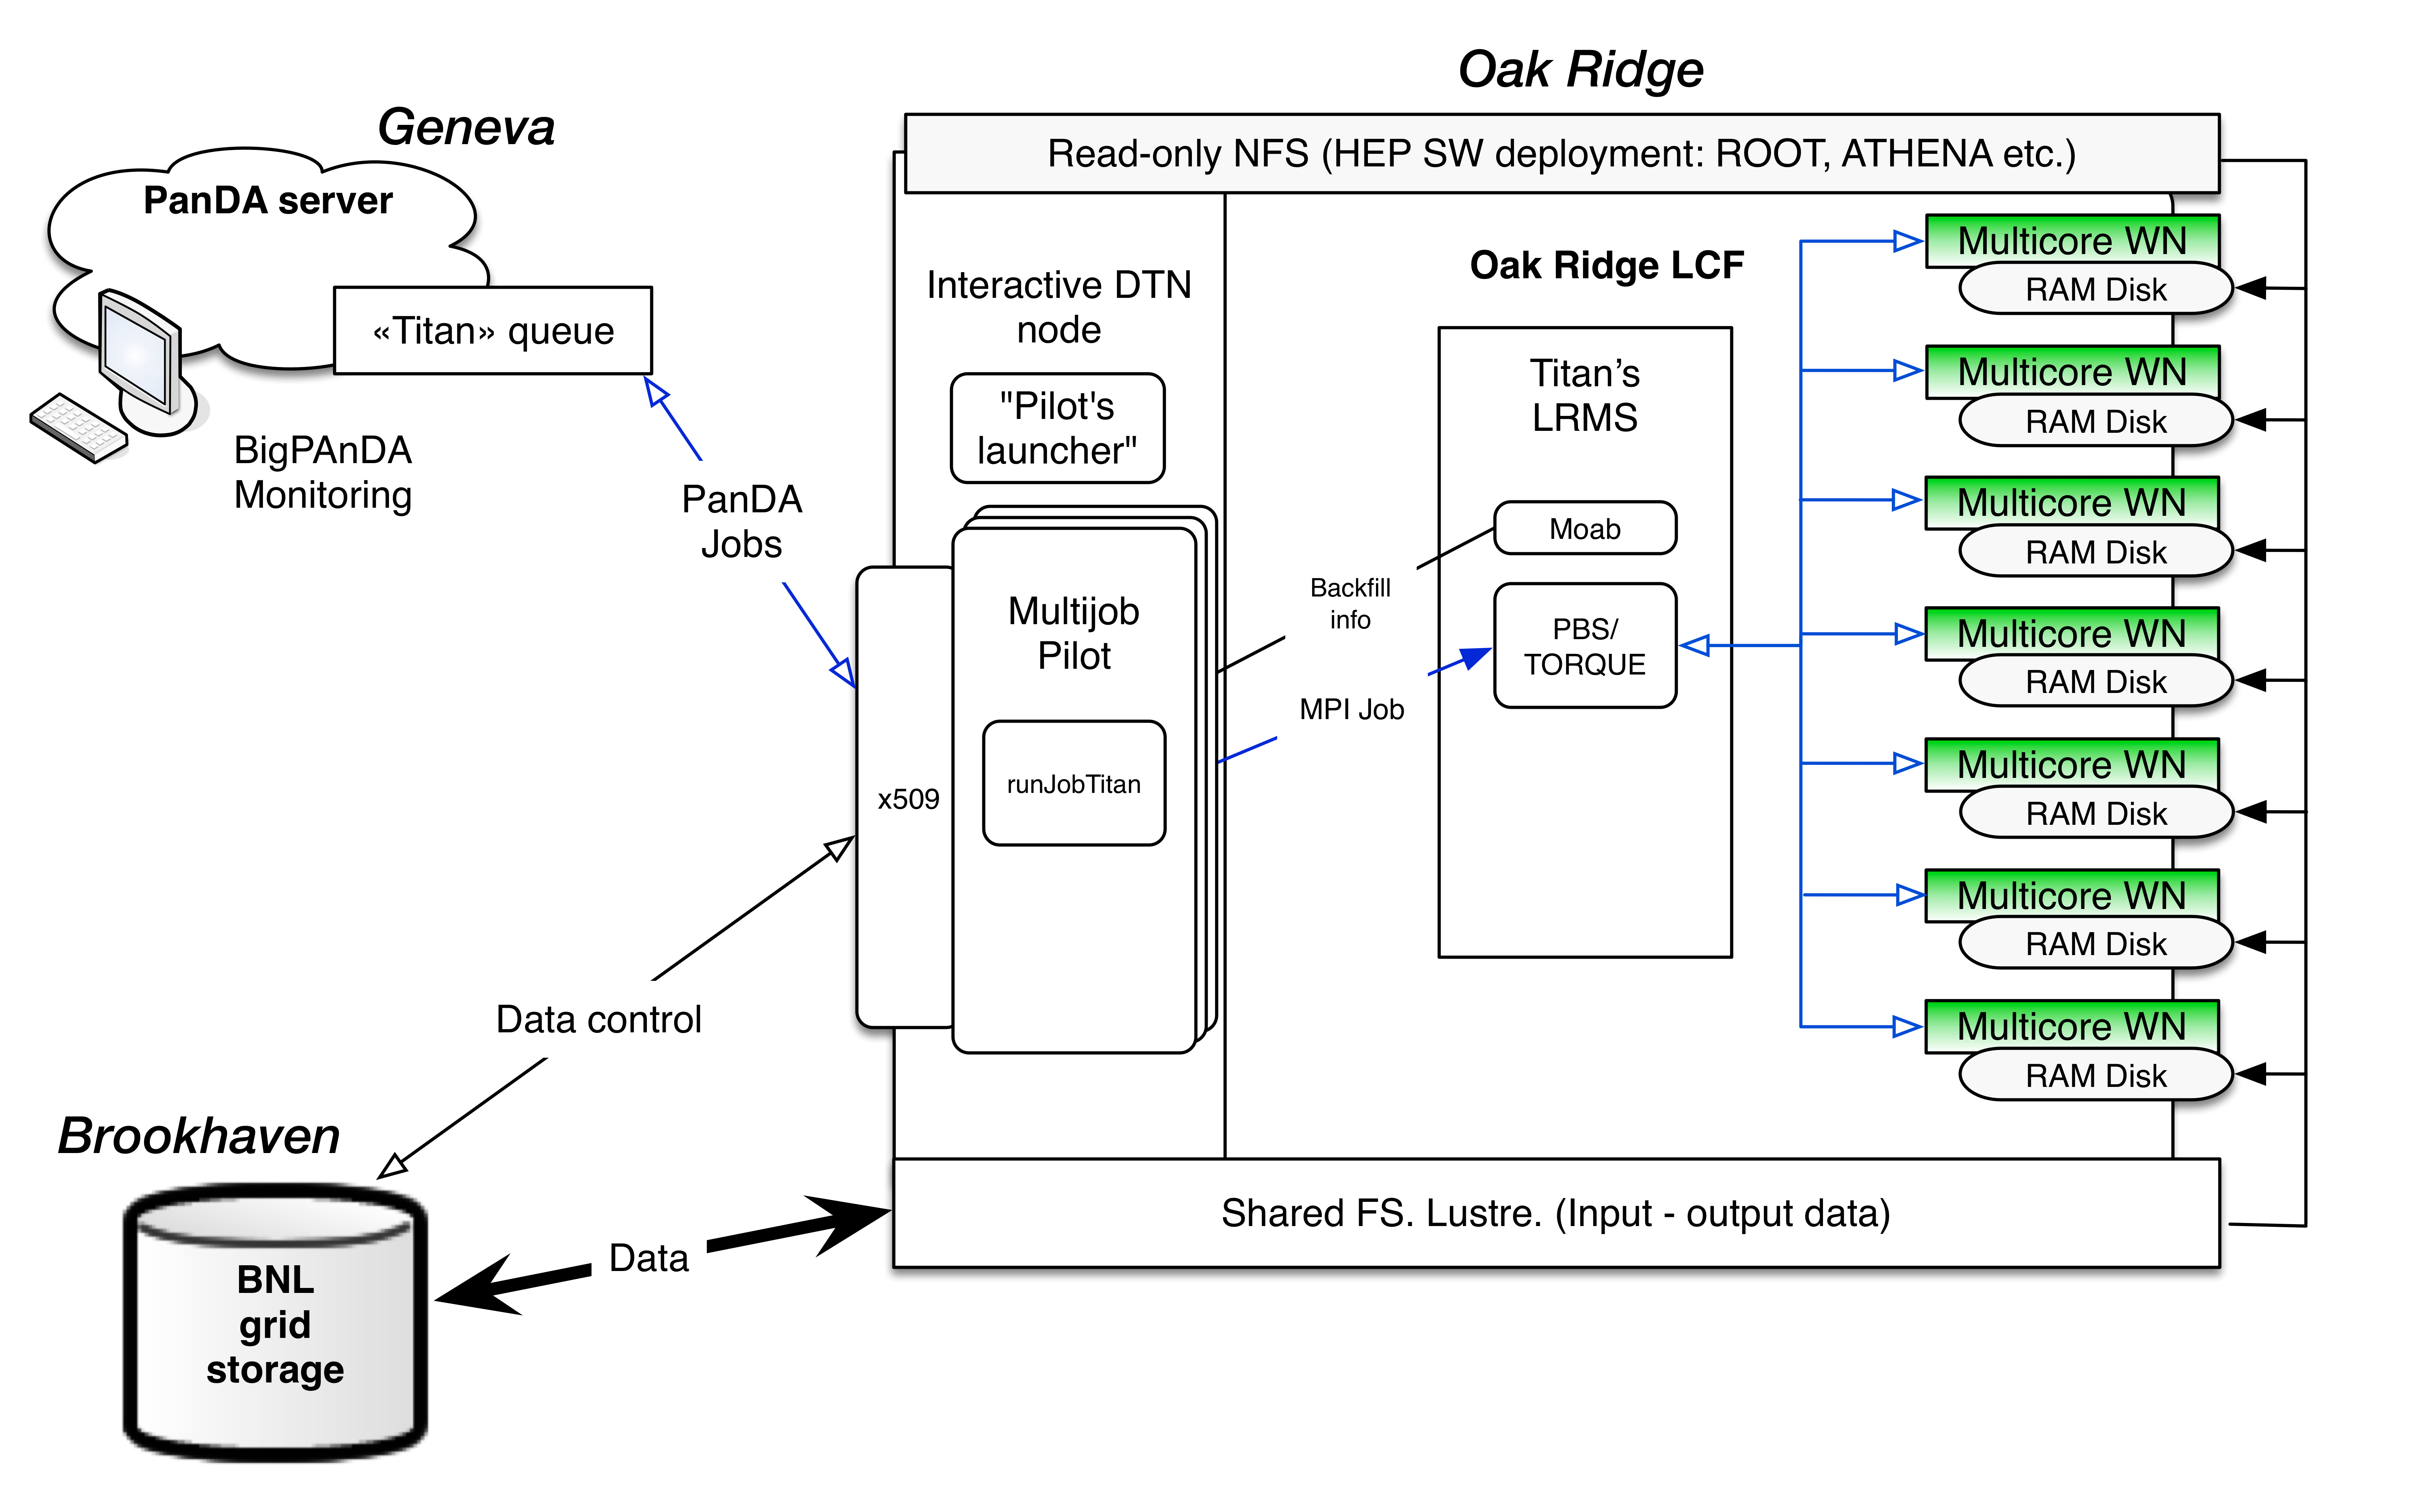
\includegraphics[width=0.75\textwidth]{images/Figure_5.png}
% figure caption is below the figure
\caption{Schematic view of PanDA WMS integration with Titan supercomputer at OLCF}
\label{fig:implementation}
\end{figure*}


% For two-column wide figures use
\begin{figure*}
% Use the relevant command to insert your figure file.
% For example, with the graphicx package use
  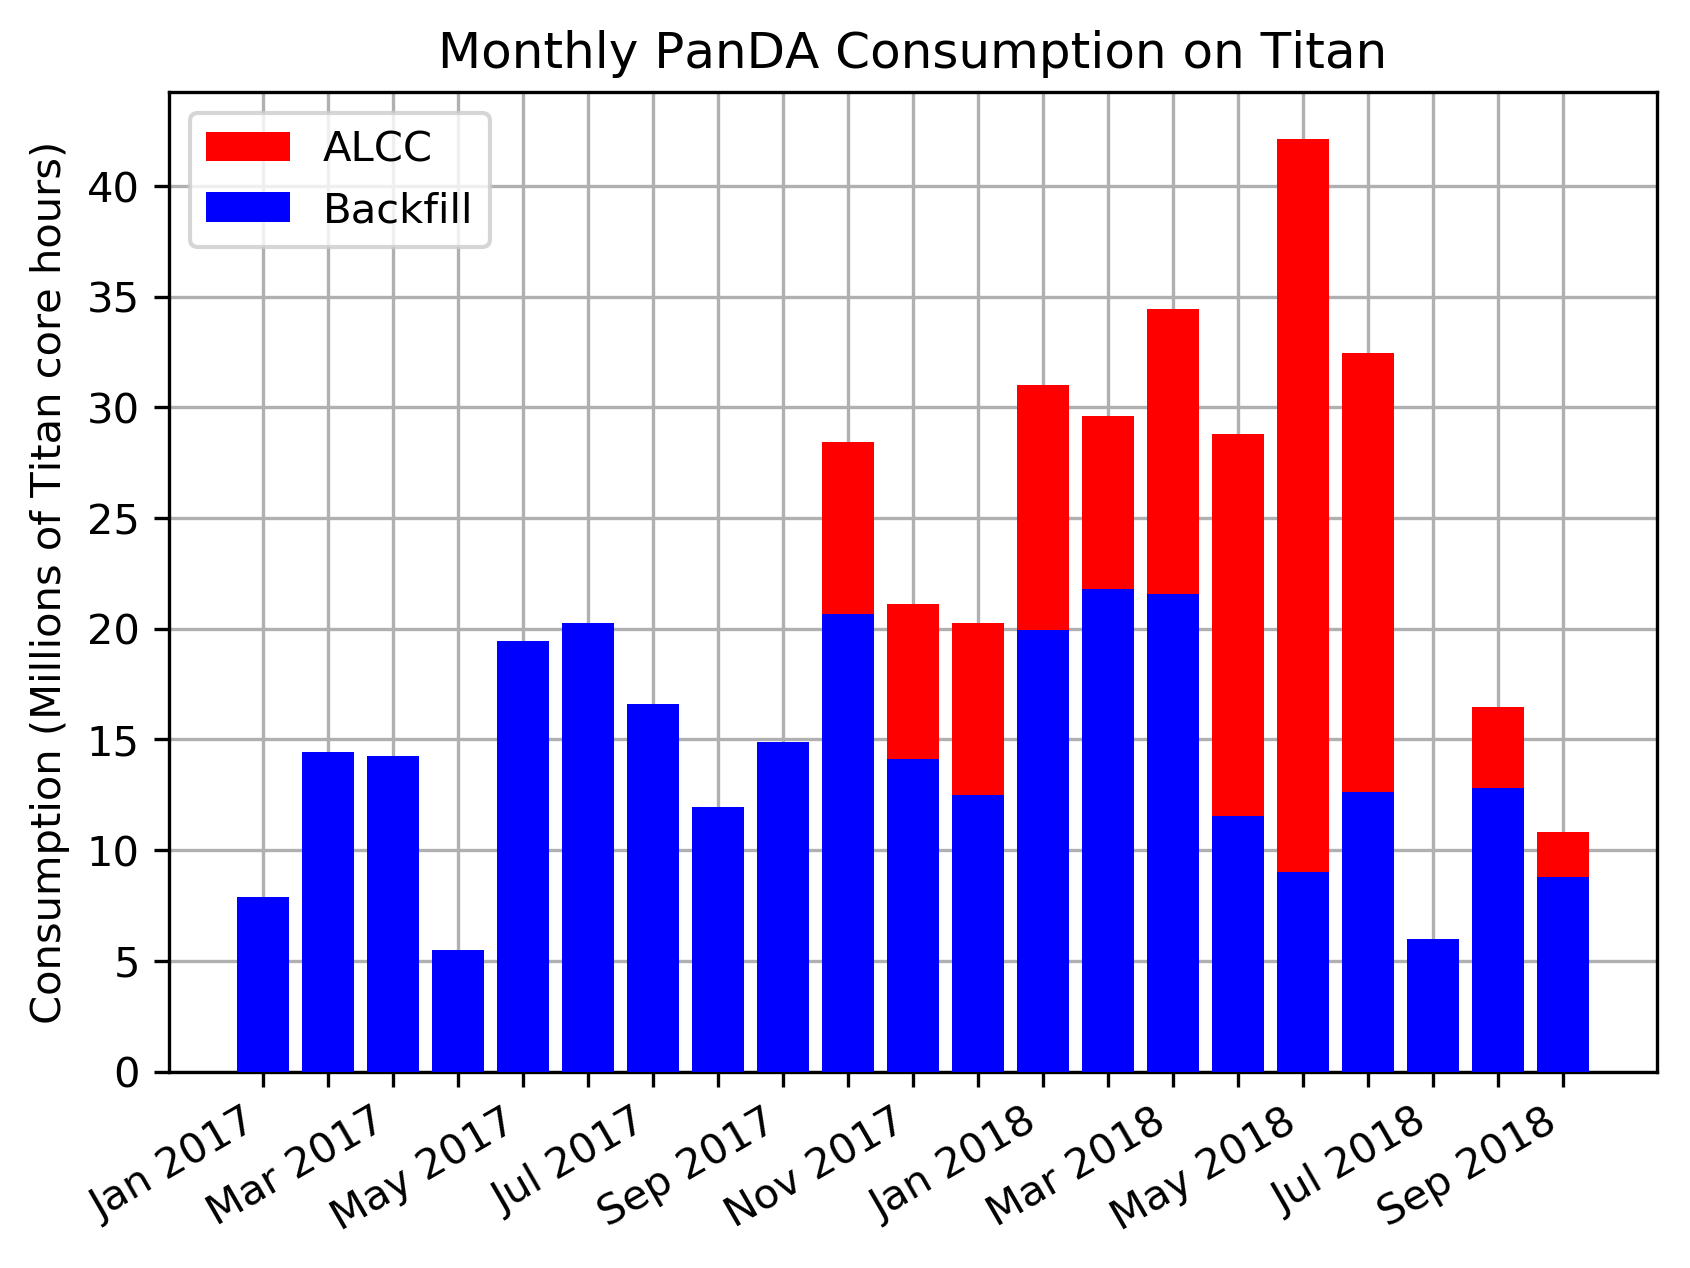
\includegraphics[width=0.75\textwidth]{images/monthly-consumption.png}
% figure caption is below the figure
\caption{This figure shows the monthly consumption of resources on Titan by the
two methods used by PanDA.}
\label{fig:monthly-consumption}
\end{figure*}

%-  vim:set syntax=tex:
